\documentclass[handout]{beamer}

\usepackage{fontspec} 
\usepackage{lsp-makros}
\useoutertheme{lsp}

\usepackage{lsptitle}

\def\two@digits#1{\ifnum#1<10 0\fi\number#1}
\def\mytoday{\two@digits{\number\day}.\two@digits{\number\month}.\number\year}


\usepackage{xspace,multicol}
\newcommand{\latex}{\LaTeX\xspace}
\usepackage{tikz}


\newcounter{lastpagemainpart}
\footnotesep0pt
\renewcommand{\footnoterule}{}
\usefootnotetemplate{
  \noindent
  \insertfootnotemark\insertfootnotetext}

\let\beamerfn=\footnote
\renewcommand{\footnote}[1]{%
\let\oldfnsize=\footnotesize%
\let\footnotesize=\tiny%
\beamerfn<\thebeamerpauses->{#1}%
\let\footnotesize=\oldfnsize}


\date{2015-04-25}

\usepackage{eurosym}  
 
\renewcommand{\centerline}[1]{\hfill#1\hfill\hfill\mbox{}}


\title{Language Science Press \& \mbox{Cross-Linguistic Linked Data}}
% \institute{FU Berlin}
\author[LangSci]{Sebastian Nordhoff \& Mathias Schenner}



\begin{document}
\lspbeamertitle
\section{Language Science Press}

\frame{
\frametitle{Language Science Press}
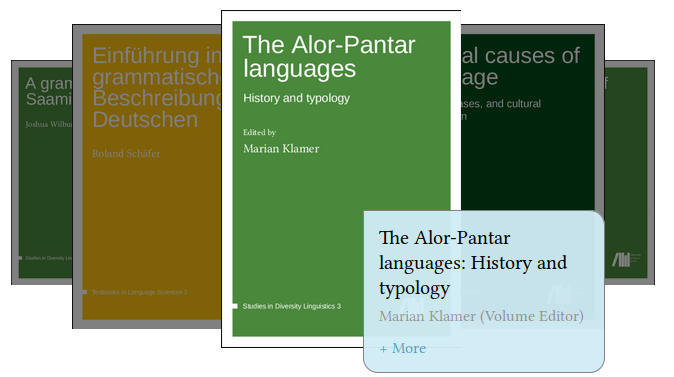
\includegraphics[height=\textheight]{catalog.png}
}


\frame{
\frametitle{Linguistische Beispiele}

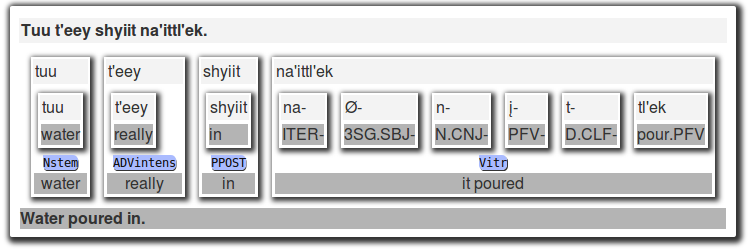
\includegraphics[width=\textwidth]{lingex.png}

\begin{itemize}
 \item Übersetzung: 
 \begin{itemize}
  \item Satz-für-Satz
  \item Wort-für-Wort
  \item Morphem-für-Morphem
 \end{itemize}
\end{itemize}

}

\section[CLLD]{Cross-Linguistic Linked Data}
\subsection[Typologie]{Typologische Datenbanken}

\frame{
\frametitle{Cross-Linguistic Linked Data\\ \mbox{The World Atlas of Language Structures}}
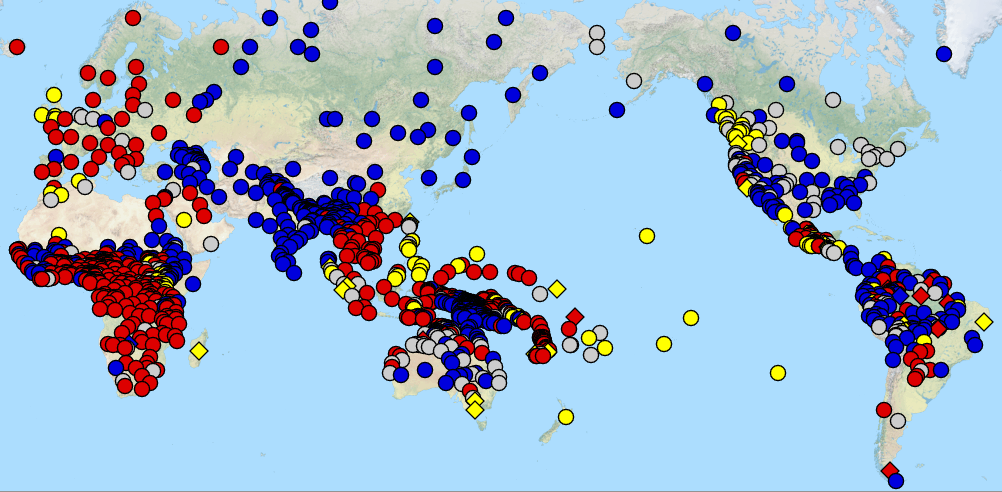
\includegraphics[width=\textwidth]{wals-sov.png}
\begin{itemize}
 \item 180 Merkmale; 2500 Sprachen
 \item hier: Wortstellung (SOV, SVO, VSO)
 \item geographische und genealogische Information
\end{itemize}

}

% \subsubsection{Apics: The Atlas of Pidgin and Creole Language Structures}
% \frame{
% \frametitle{Atlas of Pidgin and Creole Language Structures}
% 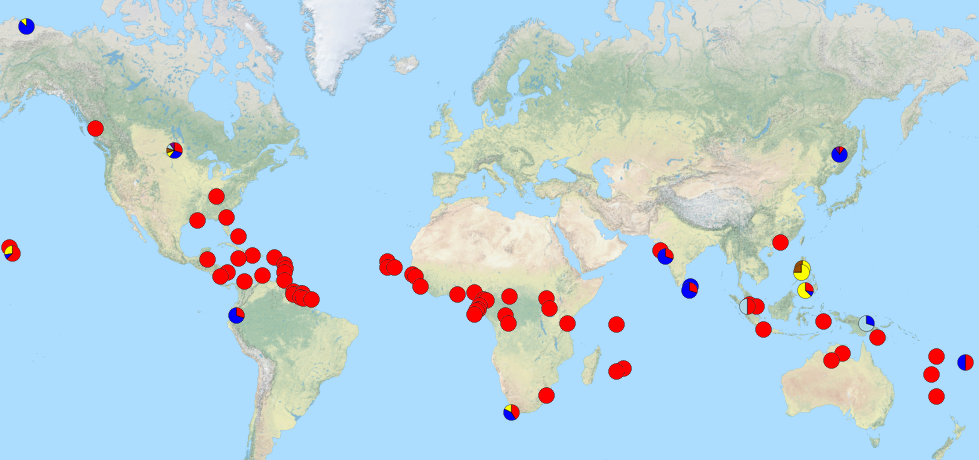
\includegraphics[width=\textwidth]{apics-sov.png}
% }


\frame{
\frametitle{Ähnliche Datensets}
\begin{itemize}
 \item \textbf{Apics} The Atlas of Pidgin and Creole Language Structures
 \item \textbf{eWAVE} 	The Electronic World Atlas of Varieties of English
 \item \textbf{SAILS} 	The South American Indigenous Language Structures 
 \item \textbf{PHOIBLE} The world's largest database of phonological inventories 	
\end{itemize}
}




\subsection[Lexikon]{Lexikalische Datenbanken} 
\frame{
\frametitle{\raggedright IDS: The Intercontinental Dictionary Series 	}

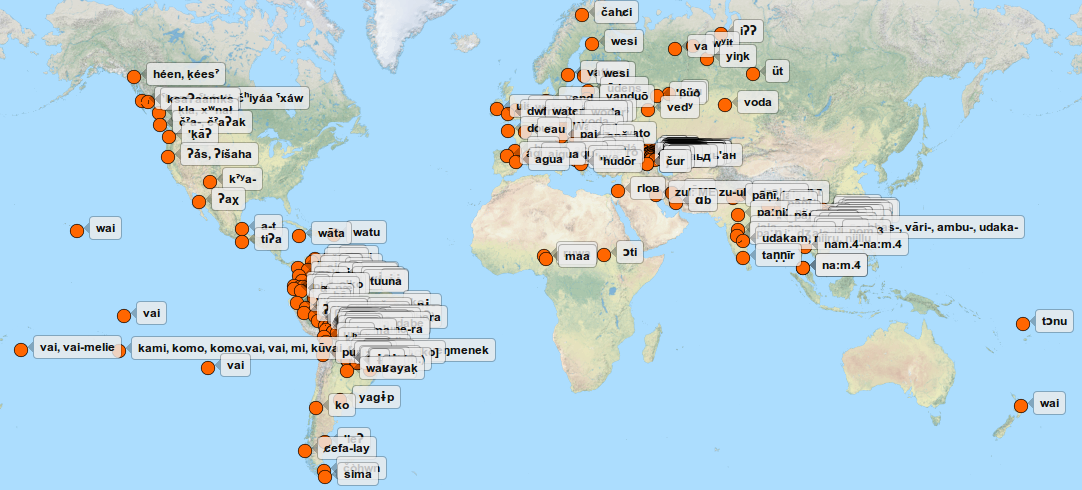
\includegraphics[width=\textwidth]{ids-water.png}

\begin{itemize}
 \item Das Wort für `Wasser' im IDS
 \item 1429 Bedeutungen; 288 Sprachen
\end{itemize}
}

\frame{
\frametitle{Ähnliche Datensets}

\begin{itemize}
 \item \textbf{Numerals} 	Numerals in the World’s Languages 
 \item \textbf{WOLD} 	The World Loanword Database 	
%  \item \textbf{ASJP} 	Lexical Database 	 
\end{itemize}
}

% 
% \subsection{Morphosyntactic databases}
% 
% \subsubsection{ValPaL}
% ValPaL 	Valency Patterns Leipzig 	
% 
% \subsubsection{AfBo}
% AfBo 	A world-wide survey of affix borrowing 	



\subsection{Literaturdatenbank}

\frame{
\frametitle{Glottolog}
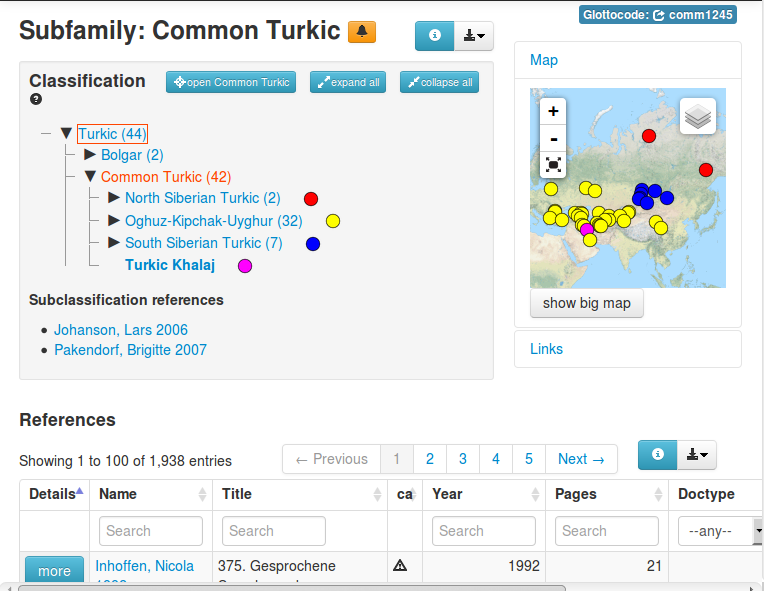
\includegraphics[height=\textheight]{glottolog-turkic.png}
}

\section{Zusammenfassung}

\frame{
\frametitle{Umfang aller Daten}

\begin{itemize}
 \item ca. 50k Beispiele
 \item ca. 500k typologische Datenpunkte
 \item ca. 25k Sprachen/Dialekte mit Klassifikation und Literaturangaben
 \item ca. 250k Literaturangaben
\end{itemize}

}
 
\frame{
\frametitle{Formate und Lizenzen}

\begin{itemize}
 \item csv
 \item xml
 \item rdf
 \item bibtex
\end{itemize}
\begin{itemize}
 \item CC-BY(-SA)
\end{itemize}

}

\frame{
\frametitle{Denkbare Anwendungen}
\begin{itemize}
 \item Wörterbuch
 \begin{itemize}
  \item Extraktion der Übersetzungen aus den Beispielsätzen
 \end{itemize}
 \item Lustiges Sprachenraten
 \begin{itemize}
  \item Zufälliger Beispielsatz
  \item Punktzahl nach genealogischem oder geographischem Abstand
 \end{itemize}
 \item Sprachenbrowser
 \begin{itemize}
  \item Aggregation aller verfügbarer Datenpunkte
 \end{itemize}
 \item Browsebare Visualisierung des typologischen Vektorraums
 \begin{itemize}
  \item \url{http://citeseerx.ist.psu.edu/viewdoc/download?doi=10.1.1.50.2428&rep=rep1&type=pdf}
 \end{itemize}
\end{itemize}


}


\end{document}
